\documentclass{article}
\usepackage{graphicx}
\usepackage[a4paper,margin=1in,footskip=0.25in]{geometry}
\usepackage{pdfpages}


\begin{document}


\title{Computer Forensics Laboratory Design}
\author{Jon Bakies \and Mitchell Dunn} 

\maketitle
\newpage

\tableofcontents
\newpage


\section{Laboratory Design}
\paragraph{} According to the NISTIR ``Forensic Science Laboratories: Handbook for Facility Planning, Design, Construction, and Relocation", a lab needs to be 700 to 1000 square feet per staff member.
The square footage per staff member approaches the low number of that threshold as the number of employees increases because shared spaces, such as reception areas and server rooms don't need to grow at the same rate as the number of employees.
With an estimated 8 staff members, this lab will require an approximate space of 6400 square feet to achieve the working goal of 800 service requests per year.

\subsection{Staff Breakdown}
\paragraph {Management - 1} 
\paragraph{} The laboratory manager is responsible for the well being of the lab.
To actively excel at their job, the manager must have general knowledge of law, computer forensics, and business.
This allows the manager to determine if the lab will be able to complete a service request based on current workload and legality. 
Most labs strive to have an ACLD/LAB accreditation status because it proves the lab follows a high standard of workplace protocol.
The manager must keep this in mind while creating policies for the rest of staff.
In order to keep evidence forensically sound a proper chain of custody record has to be met and the evidence has to be properly handled while being investigated.
These policies will not only improve the efficiency of the lab, but will also improve workplace ethics.
\paragraph{Lawyer - 1} 
\paragraph{} The Lawyer will act as a consult for the Computer Forensics staff to ensure all evidence is extracted legally and to verify the evidence is usable.

\paragraph{IT Specialist - 2}
\paragraph{} The IT Specialists will focus on the internal network and security of the lab.
The IT Specialist should have 5 years experience as a system administrator, and be well versed in security.
The IT Specialists will be in charge of securing the hardware and evidence and managing access to the network hardware.
They should follow ACLD/LAB policies for lab and equipment security.
The IT Specialist will also act as a system administrator managing users, limiting communication between VLANs, hosting evidence to be easily accessed by authorized personnel, and maintaining the network for the Laboratory.

\paragraph{Computer Forensic Investigator - 5}
\paragraph{}  A computer forensic investigator should have the skills needed to extract evidence from a device in a non damaging and legal way.
It is important that the team of investigators are experienced in varying devices to enable the lab to accept a wide range of service requests.
Evidence and other information can be from from any electronic device, ranging from laptop and computers to mobile phones and game consoles.
All of these devices have their own operating system, meaning the investigator needs know how to work with multiple operating systems and software.
\subsection{Laboratory Layout}
\subsubsection{Office Space}
\paragraph{} The office space is designed to be the seating for the entire staff.  
The desks have privacy walls so employees can work in peace, but the desks are in the same room to allow for cooperation.  
Each desk will hold the staff members workstation and will also have a dedicated power supply to keep workflow alive and to prevent the loss of sensitive data in the rare case of a power outage. 

INSERT INFO ABOUT WORKSTATION HERE

An IP phone will complete each desk so staff members can conduct business with people outside of the office.
Under each desk is a small opening to a trough for cable management.
This room contains the only entrance into the rest of the lab, meaning the main door needs to have some hefty security
The door will be a double wide door made out of 18-gauge steel.
The lock on the door will be controlled by an RFID badge and key code entry.
\subsubsection{Conference Room}
\paragraph{}
The conference room is a large room with a table and plenty of seating.  
A forensic laboratory conducts a fair amount of business, mostly with the clients it takes in.
This room can be used for a multitude of purposes including staff training, planning an investigation, and meeting with clients.
A TV on the wall will assist with presentations.
The network can only be accessed wirelessly while in the conference room.
This limits the kind of work that can be done in the conference room.
Because there are no sensitive devices or information in the conference room, there will not be a lock on the door into the conference room.

\subsubsection{Server Room}
\paragraph{}
This room contains the most sensitive part of the network, meaning this room has the strongest security in the building.
The door into the server room will have the same RFID badge and key code lock as the main door, but access will be limited to only those who are authorized.
The server is a critical part of the lab, as it is controls all of the data traffic coming to and from the lab.
To ensure the safety of the server, this room has its own air supply unit and control to keep it at a temperature and humidity level that is safe for the hardware.
The room will have antistatic epoxy flooring, and the handlers are instructed to wear antistatic wristbands connected to the case of the server rack to protect the internals from electrical damage.
To keep the server runner and have a redundant power supply, there will two mounted within the server rack.
To connect the rest of the lab to the network, there are a couple troughs running below the floor.
This trough is designed with security in mind.
There is no access to the trough from outside of the building, and is far too small to allow access into the server room.

\subsection{Workbench}
\paragraph{}
Forensic investigators often need to disassemble hardware and copy disk drives to gather the evidence needed for the investigation.
The workbench will act as an area for the investigators to work on the physical devices.
In the area around the workbench there are locked cabinets to house the tools and equipment needed to work on varying devices.
The investigators have an open desk to place and disassemble the hardware, documenting each step of the way.
A trough underneath the bench supplies a couple connections to the network to enable the investigator to work on their workstation while at the bench.
Lab policy enforces the investigators properly document the process they take to keep chain of custody intact, store the evidence in a secure place, and to return hardware in the same status is was received.
The prevent damage done to hardware, the workbench is covered with antistatic mats, and only properly trained investigators will work on the hardware.
The workbench is locked in a room with the evidence locker, storage locker, and contains the only entrance to the server room.
The workbench is locked with an RFID badge and key code lock that can limit access to those who are authorized.

\subsection{Evidence and Storage}
\paragraph{}
Proper evidence handling and storage is one of the policies that is needed to get an ACLD/LAB accreditation.
Evidence is placed in heat sealed antistatic bags, to prevent tampering and electrostatic discharge.
Properly bagged and labeled electronics are then stored in a 16 gauge steel, anti pick locker.
These lockers are caged in a floor to ceiling fence in the same room as the workbench.  
To access the lockers, a person needs to access the building, the work bench room, and finally into the fenced in area which is locked with the RFID reader and key code.
Storage for lab equipment is stored in the same fashion, but partitioned in a separate cage from the evidence.


\subsection{Figures}
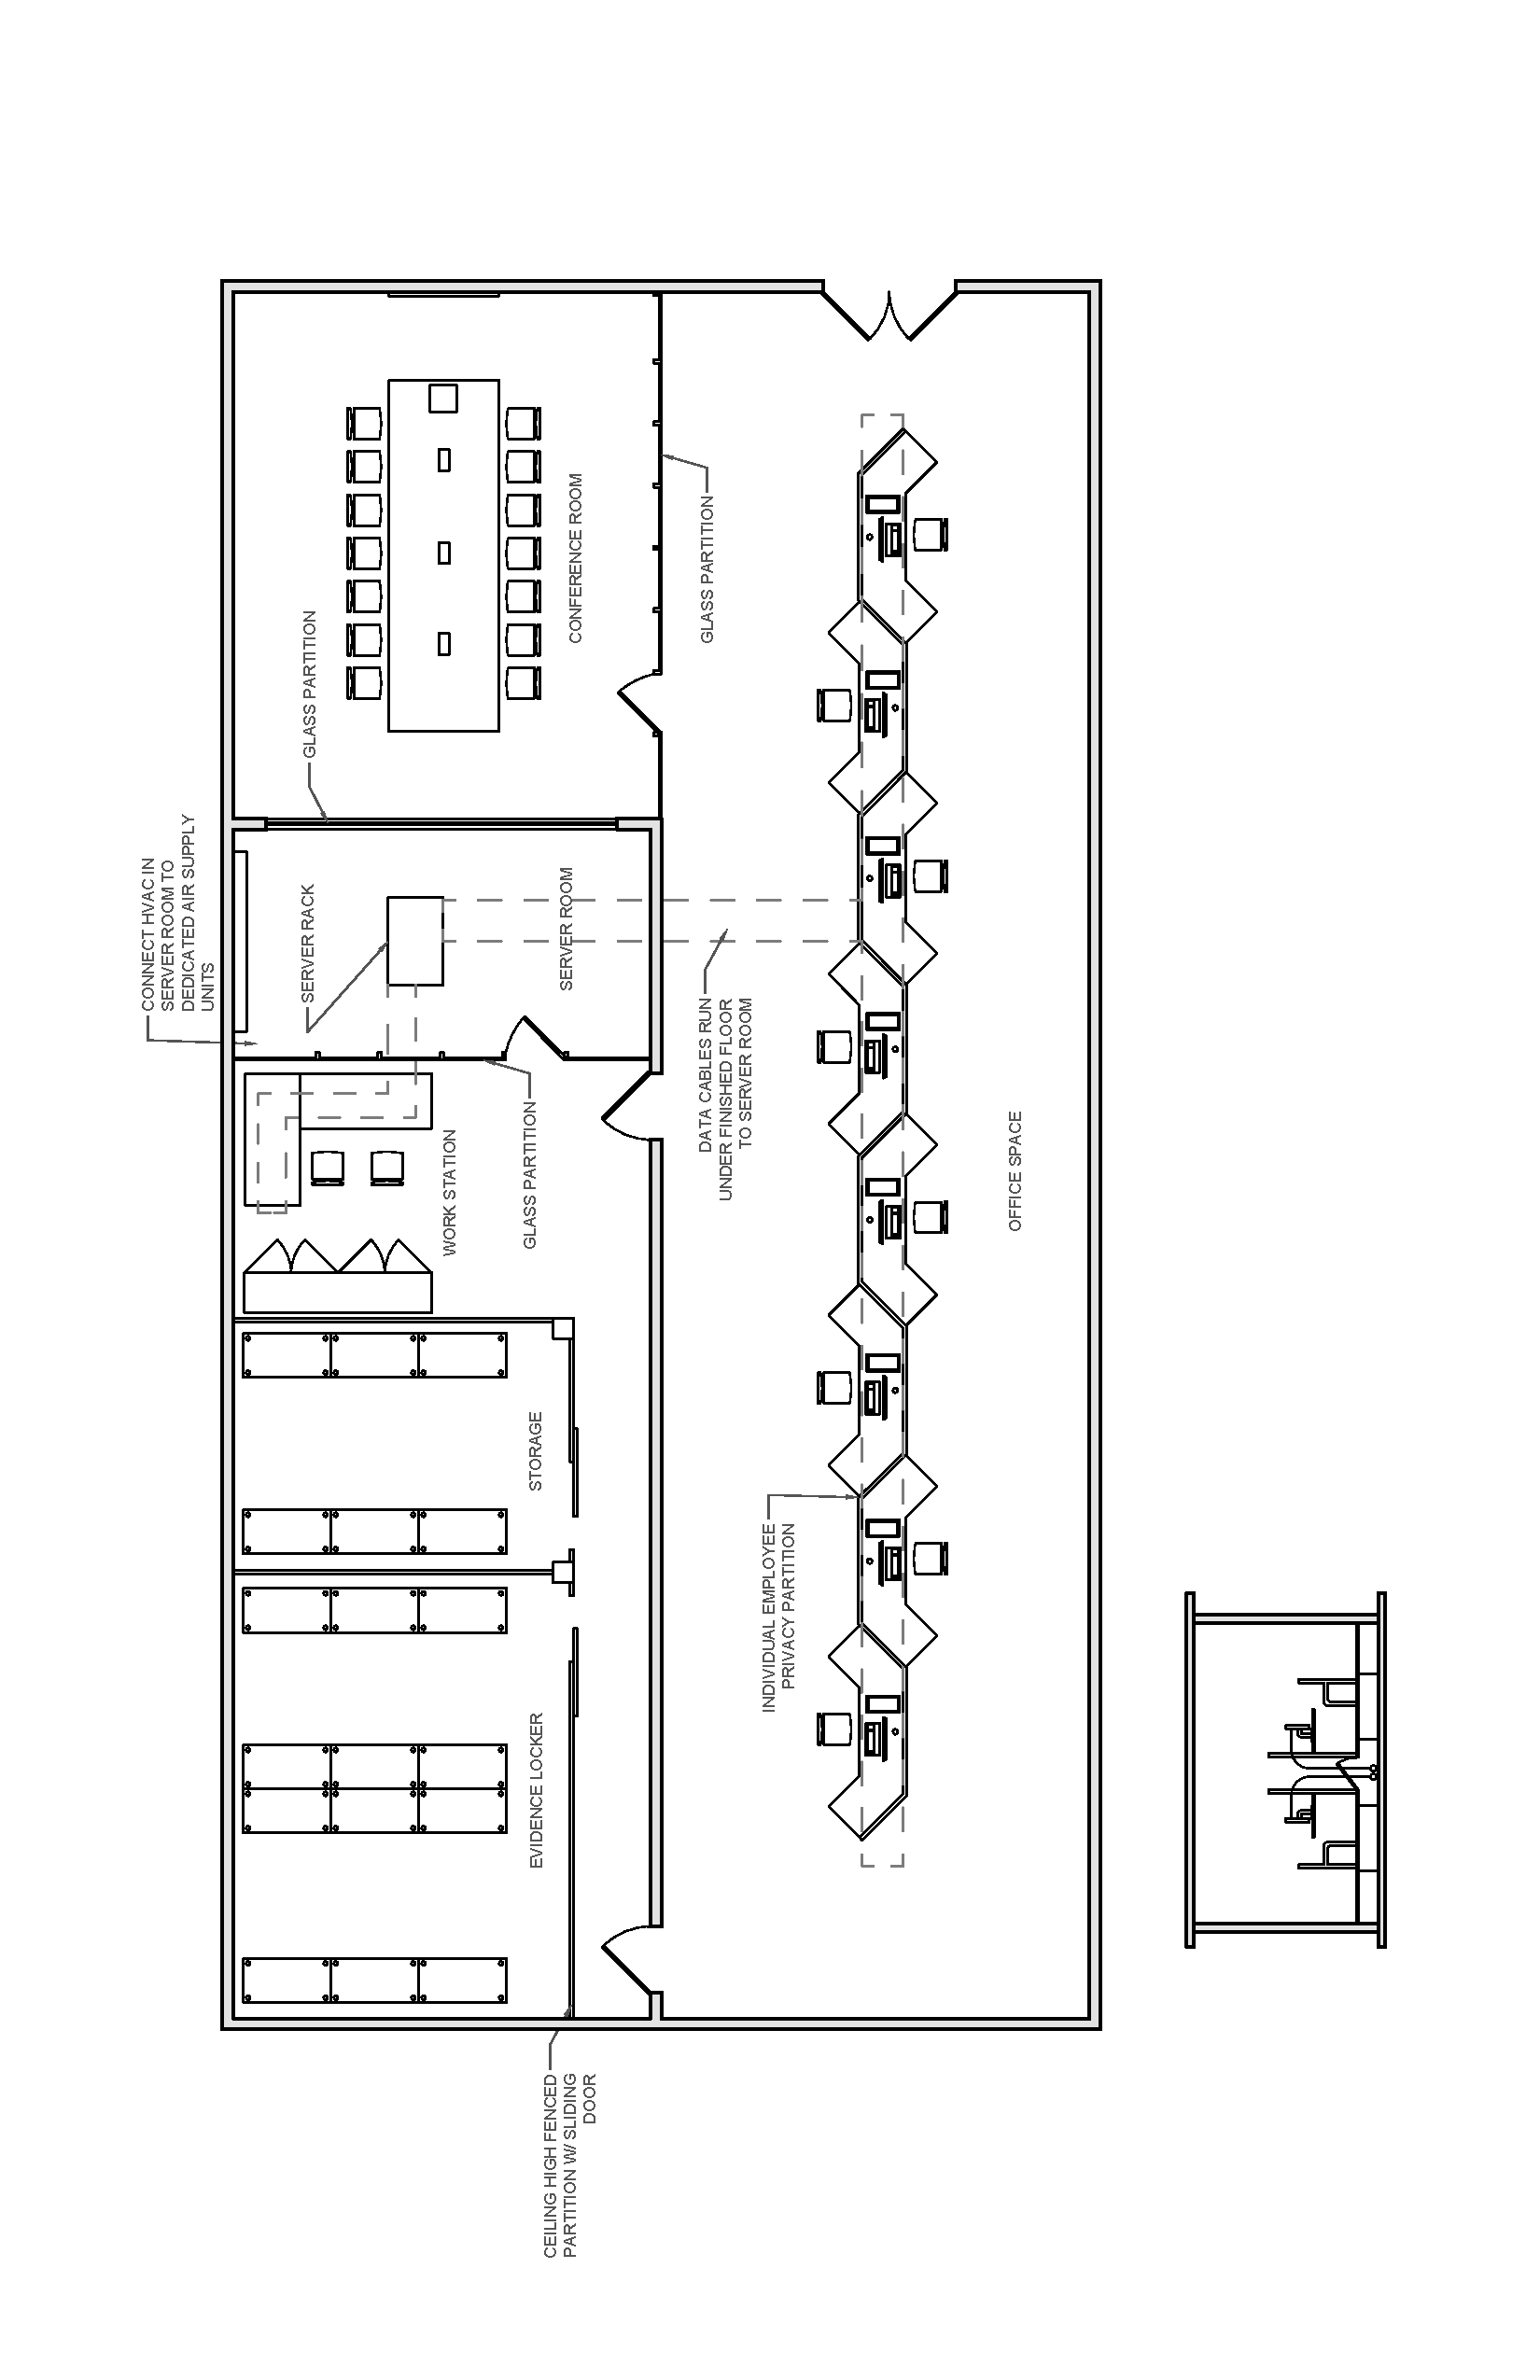
\includepdf[pages=-, angle=180]{layout-thx-nick-millet.pdf}
\section{Hardware}
\subsection{Employee Laptops} 
\subsection{Tools for Employees} 
\subsection{Server Rack}
\subsubsection{Power Supply} \paragraph{} The power supply to the server rack should be through an uninterruptible power supply (UPS) in order to ensure that the power supplied is clean and backed up by a battery.
The UPS should have enough capacity to run for the time it takes to start a diesel generator to take over as the power supply.
The diesel generator should have monthly testing, as well as the power supply failover operation.
Each system in the rack should have two power supplies to help guarantee uptime.
Each leg of the system should be plugged into a different rack mounted power supply to allow a power supply failure.
 
\subsubsection{Networking} \paragraph{} The networking would be simple, one 48 port switch would be sufficient for the entire network.
And the connection to the ISP would be connected to a Router/Firewall box.
The connection to the ISP should be fiber and have an uplink of at least 500Mbps to ensure that employees can connect remotely and download large files without saturating the link for a long time.
A second connection to a different ISP should be considered, to be used as a failover in case of maintenance to the first ISP.
To improve security further on the ISP link a Network Detection and Response, such as RSA's NetWitness system would be running on the internal virtual machine cluster described below.
Each virtual machine would need three uplinks, one to the employee local area network, one to the Storage area network, and one link for VMWare.
These networks will be isolated from each other using VLANs in order to enhance security.
Other VLANs could be implemented to further isolate network devices like IP Cameras and smart door locks to prevent people from directly accessing and potentially compromising them.
A wifi access point connected to the switch and 802.1x to authenticate to Active Directory to ensure only employee devices are connecting.
Another vlan and separate wireless network, even on the same physical access point, with a password could also be provided to convenience the employees by providing wifi to their personal devices (e.g. personal cellphones).
The convenience network would have very strict firewall rules and would not pass traffic to any of the other networks.

\subsubsection{Virtual Machine Cluster} \paragraph{} The purpose of the virtual machine cluster is to provide investigators with multiple computers in the most convenient way possible.
Since investigators should have access to any operating system they could would need at any time instantly, it is expected that each investigator will have three to five virtual machines at any time.
In addition to investigators the IT staff might also want to run some virtual machines for their convenience.
This cluster will also provide infrastructure for internal and external services.
Internal services would include Active Directory, samba/NFS/FTP sites, etc.
Active Directory would be the central authentication for all the services.
The cluster would be at least four Dell R630s or an equivalent from another company.
If the capacity allows it VMWare's high availability features can be leveraged to run multiple copies of the same virtual machine for critical infrastructure like the Windows Domain Controller in order to ensure that even if a physical host powers off unexpectedly the domain controller would continue to operate and employees are not interrupted.
For cases where video processing is involved graphics cards can be installed on the virtual machine hosts and using PCI passthrough to attach graphics cards to the virtual machines to greatly enhance their video performance.
This would allow investigators to comforatbly work from their laptop and still have the benefits of full size, powerful graphics cards.

\subsubsection{Storage} \paragraph{} 


\section{Software}
Software required for the lab to act as a function Forensic Lab.

\end{document}
